\chapter{Introducción}

Este proyecto nace con la intención de trabajar sobre el proyecto de código abierto Pyomo \cite{pyomo}, y aportar una implementación paralela de su módulo de resolución de problemas mediante programación estocástica. El objetivo es que la aplicación pueda resolver problemas de mayor tamaño en un tiempo razonable aprovechando el uso de computación distribuida.

\section{Pyomo y la Programación Estocástica}

% Explicar el proyecto Pyomo, que resuelve muchos tipos de problemas. Ver la motivación original del proyecto. 
% Programación Estocástica, tipos de problemas y aplicación en el mundo real.

Pyomo \cite{pyomo} es un paquete de software basado en Python destinado a la formulación y solución de modelos de optimización. Fue desarrollado por \textit{Sandia National Laboratories} y \textit{University of California, Davis} y permite la solución de multitud de problemas distintos, permitiendo su utilización con multitud de solvers de terceros como CPLEX \cite{cplex} o GLPK \cite{glpk}. Pyomo es un proyecto extensible mediante la integración de plugins que pueden ser programados por la comunidad para uso privado o público gracias a su filosofía de código abierto.\\

En este proyecto se ampliará el módulo PySP, el paquete de Pyomo dedicado a la solución de problemas estocásticos. La Programación Estocástica \cite{stochasticProgramming} resuelve problemas de optimización donde existe un cierto grado de incertidumbre. Esta incertidumbre hace que no podamos pensar en un problema como algo estático. Los distintos valores posibles generarán escenarios diferentes y, si contamos con varias variables inciertas y dependencias entre ellas, podemos tener un problema que se desarrolle en más de una fase. Por esto, este tipo de problemas suelen representarse como un árbol donde cada nodo es un posible escenario.\\

\begin{figure}[H]
    \centerline{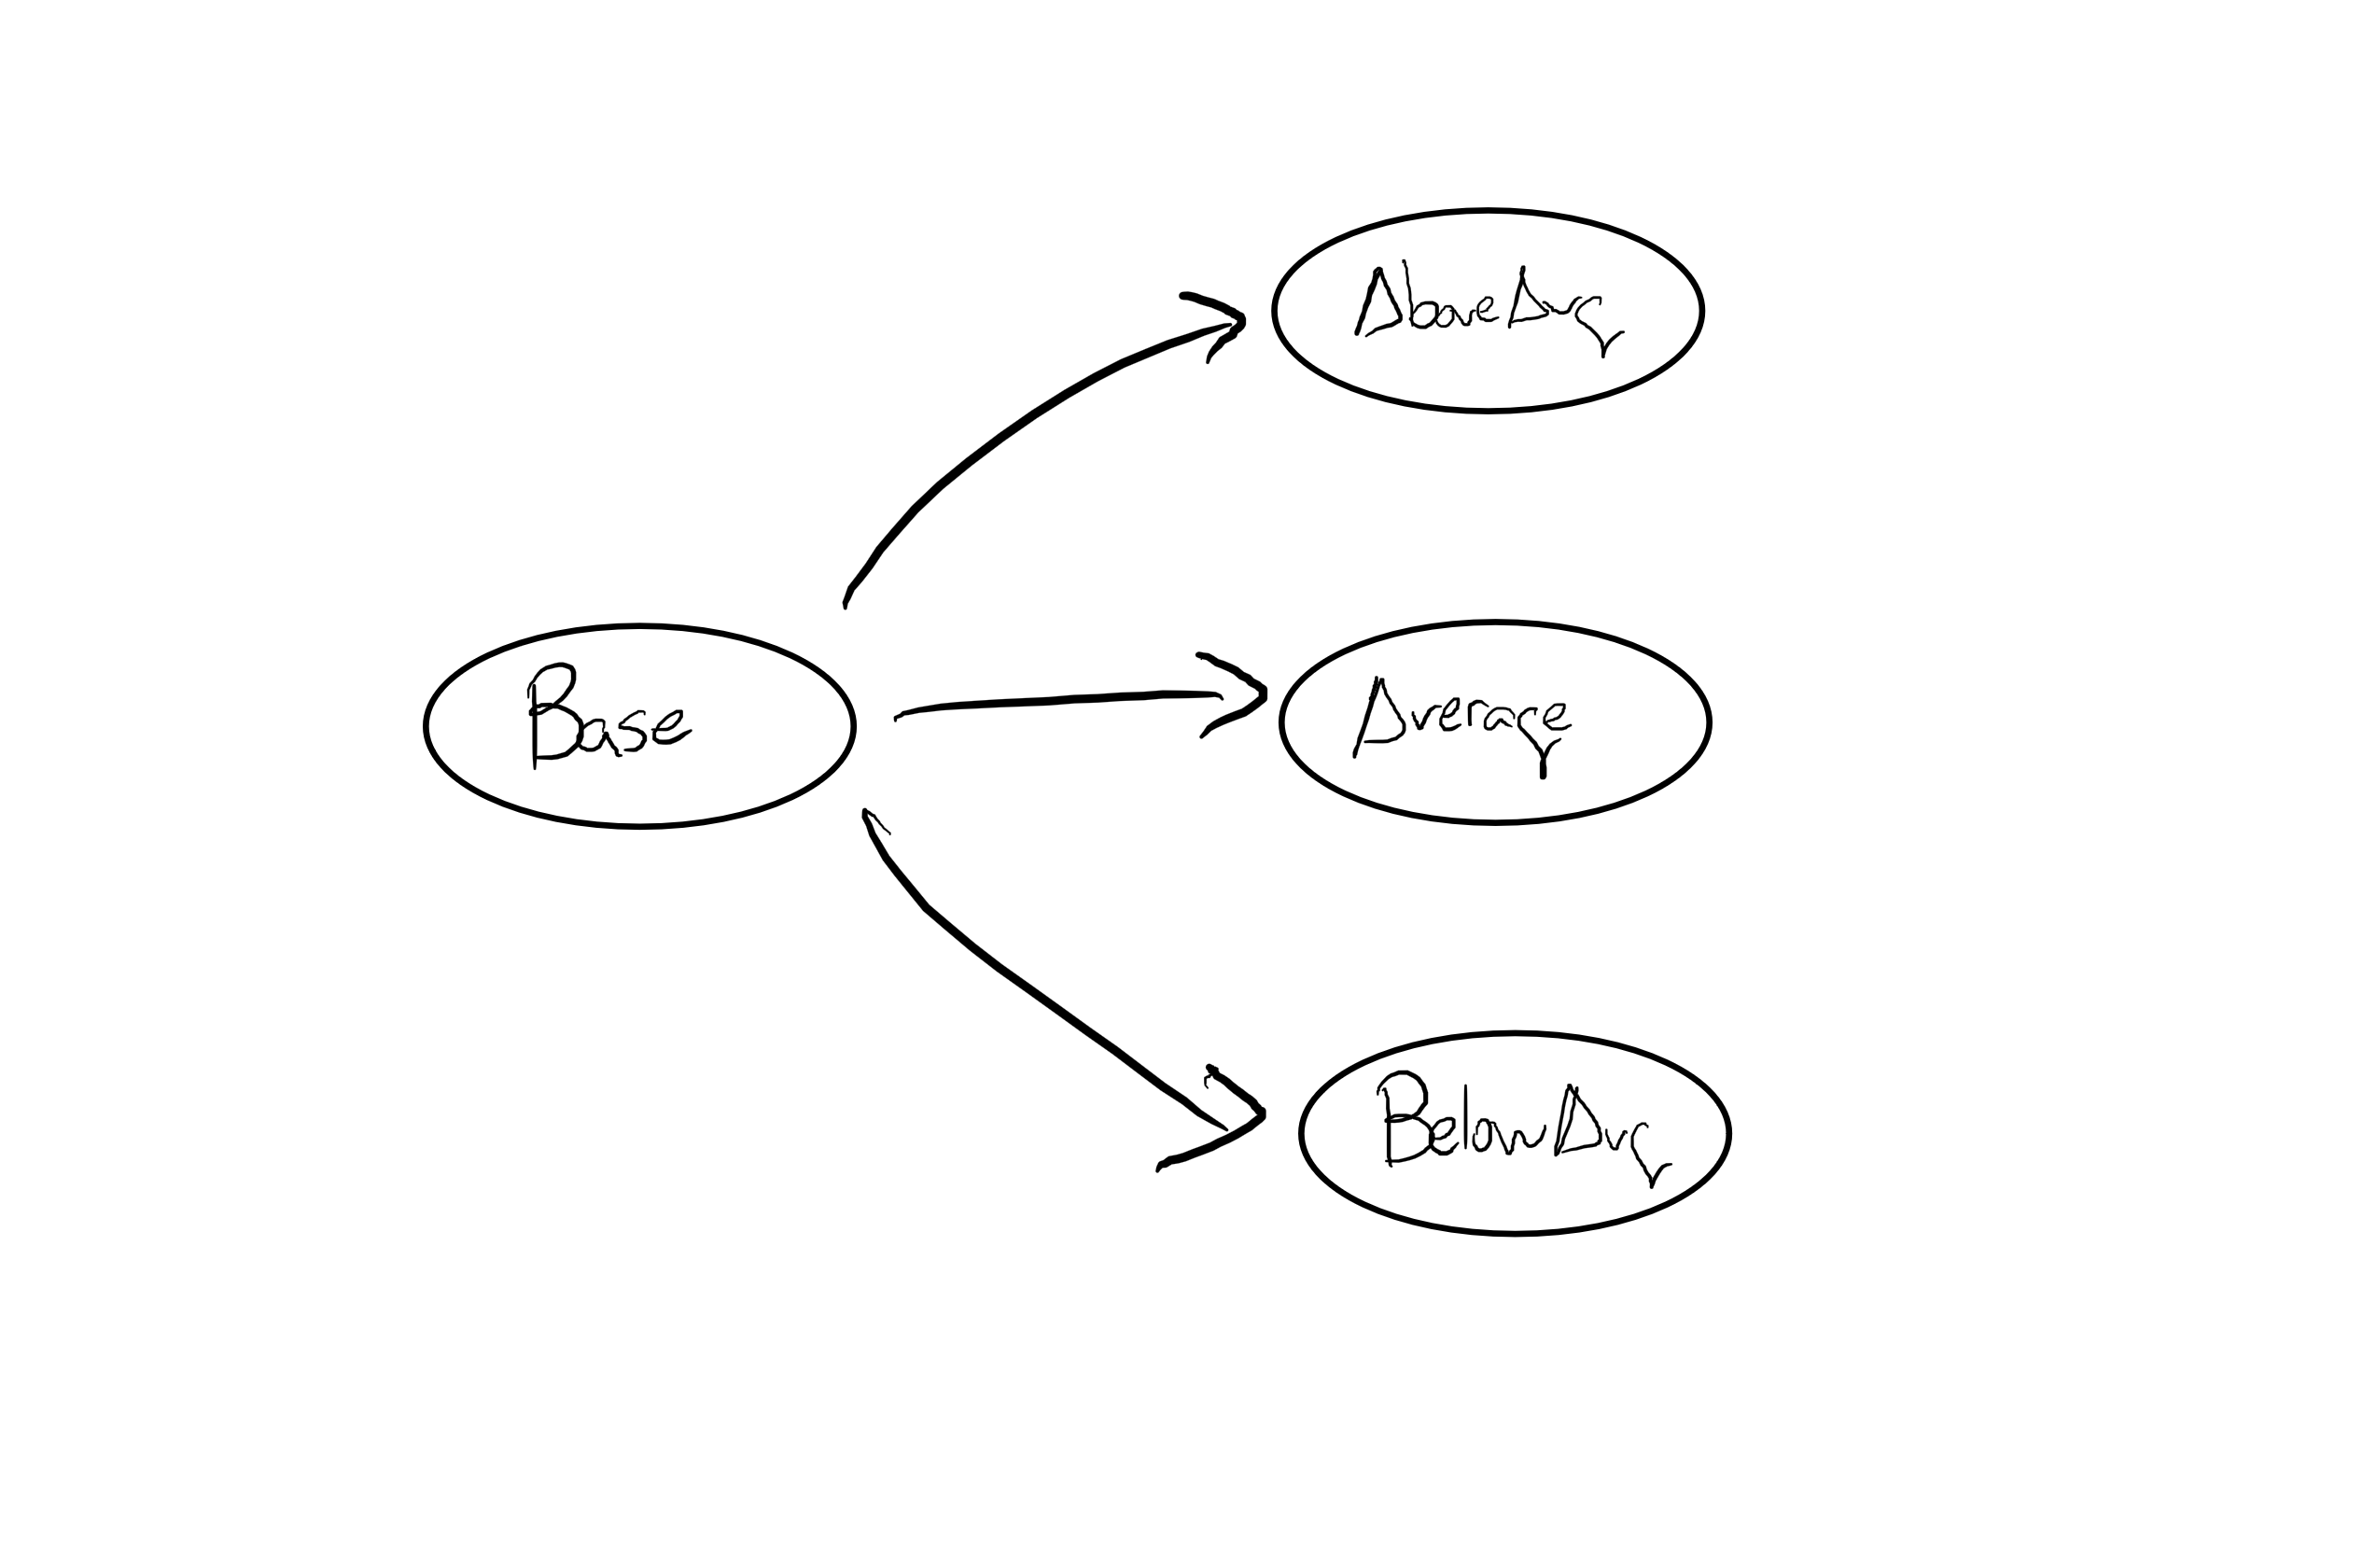
\includegraphics[width=15cm]{figuras/scenario-tree.png}}
    \caption{Árbol de escenarios en un problema estocástico}
    \label{fig:scenario-tree}
\end{figure}

% TODO: Buscar un mejor ejemplo
Este tipo de problemas es muy común en el mundo real. Por ejemplo, en una tesis defendida en la Universidad de Chile \cite{thesisHydro}, se utiliza la programación estocástica aplicada a la coordinación hidrotérmica. Este problema ``busca encontrar la operación óptima para un Sistema Eléctrico Mixto, combinando en la solución los efectos de las etapas futuras así como los efectos que la hidrología tiene en la operación del sistema''. Es un problema de optimización para una red energética gubernamental donde se deben tener en cuenta costes y eficiencia de cada tipo de generación de energía, además de contar con factores externos. \\

Los problemas estocásticos pueden subdividirse en problemas individuales (un problema para cada combinación de posibles escenarios generados) lo que los hace muy buenos candidatos para su paralelización. Estos problemas individuales deben converger a una solución única, lo que se consigue con un algoritmo como el \textit{Progressive Hedging} \cite{progressiveHedging} el cual hace uso de las variables concretas de cada escenario y el valor de control $\rho$ para hacer converger las soluciones a un valor equivalente a la resolución del problema antes de subdividirlo.

\section{Motivación del proyecto}

% Adaptarse a nuevas tecnologías para abarcar problemas de mayor tamaño.

Como se ha explicado en el apartado anterior, los problemas estocásticos representan situaciones comunes y su solución puede ser aplicable a muchos campos diferentes. Además, Pyomo ya dispone de herramientas para solucionar este tipo de problemas de forma sencilla, siendo incluso posible hacerlo de forma paralela.\\

Este proyecto tiene como objetivo realizar una nueva implementación alternativa haciendo uso de herramientas Big Data como Spark \cite{spark} o modelos de programación clásicos como MPI \cite{mpi}. Esta implementación funcionará como base para la resolución de problemas estocásticos en entornos distribuidos, siendo susceptible de recibir optimizaciones concretas para la tecnología escogida y plataformas futuras.

\section{Estado del arte}

% Hablar de Big Data, su orientación principal al manejo de datos masivo. Haremos una adaptación a usarlo como motor de cálculo en entornos de computación distribuida.

Existen múltiples métodos para solucionar problemas estocásticos. Una forma es solucionar la ``representación extendida'' del problema. En este caso se preprocesa el árbol de escenarios para resolverlo como un problema único.\\

El método en el que se centrará este proyecto es el algoritmo \textit{Progressive Hedging} (PH) que, como se explicó anteriormente, consiste en la solución de subproblemas y la convergencia de sus soluciones. Podemos ver el pseudo-código del algoritmo concreto en la \autoref{fig:ph_pseudocode}.\\

A continuación se especifican las posibles herramientas para implementar este algoritmo y Pyro, la librería utilizada en la implementación paralela ya existente en Pyomo.

\subsection{Tecnologías Big Data}

El término Big Data se refiere al manejo masivo de datos cada vez más relevante en los últimos años. El software orientado a Big Data está optimizado para la obtención, almacenamiento y procesamiento de grandes cantidades de datos que sería inviable analizar con software tradicional. \\

Estudiaremos la herramienta Spark \cite{spark} de Apache para la implementación del algoritmo. Spark es un framework de código abierto para la programación en entornos distribuidos. Proporciona una capa de abstracción que permite ejecutar trabajos de forma distribuida sin tener conocimiento de las características del cluster. Spark se encarga de la distribución de los datos, el mantenimiento de su consistencia y la optimización de la repartición.\\

\subsection{MPI}

MPI, siglas para \textit{``Message Passing Interface''}, es un estándar de paso de mensajes que permite la comunicación entre programas a través de la red. Esta interfaz puede utilizarse para implementar una red de objetos distribuidos y solucionar problemas de forma paralela.\\

MPI permite el paso de mensajes utilizando tipos primitivos o la creación de tipos personalizados. La comunicación puede ser punto a punto entre dos objetos, sincronizando las llamadas a \textit{send} y \textit{receive}, o puede ser colectiva. MPI también provee funciones para facilitar la ejecución de algoritmos distribuidos como MPI\_BCAST, MPI\_SCATTER o MPI\_REDUCE.\\

Dado que MPI es un estándar, existen librerías para multidud de lenguajes de programación diferentes. Esto permite que programas escritos en lenguajes diferentes puedan colaborar usando una interfaz común. Una utilidad de esta interoperabilidad es poder escribir un nuevo programa que ejecute trabajos en un lenguaje moderno y que se comunique con un programa anterior sin tener que modificarlo. \\

MPI define una interfaz de bajo nivel para ejecutar trabajos en paralelo. Esto permite una mayor optimización pero debemos ser más cuidadosos con la implementación. Si queremos paralelizar un programa debemos gestionar manualmente la división de la memoria así como sincronizar los mensajes enviados y recibidos.
 
\subsection{Pyro}

La intención de este proyecto es realizar una implementación paralela del algoritmo \textit{Progressive Hedging}. Para cumplir este objetivo satisfactoriamente, debemos fijarnos en la implementación existente que, en este caso, utiliza la librería Pyro \cite{pyro}. \\

Pyro es una librería de Python para la implementación de objetos remotos. Funciona de una forma similar a RMI de Java, utilizando un servidor de nombres donde los objetos son registrados. Una vez hecho el lookup de un objeto remoto se puede utilizar como un objeto nativo de Python, pero la ejecución se realizará sobre el objeto remoto.\\

Este tipo de comunicación entre objetos permite adaptar de forma sencilla un algoritmo implementado con una arquitectura basada en objetos a un entorno paralelo. Sin embargo, este tipo de comunicación tiene ciertas desventajas:

\begin{itemize}
    \item Se debe gestionar manualmente la repartición de trabajo en un entorno distribuido.
    \item No es sencillo optimizar la distribución de memoria entre los nodos de trabajo.
\end{itemize}

\section{Objetivos}

% Los objetivos expuestos en el anteproyecto: generar un módulo para Pyomo y evaluar su rendimiento.

El objetivo principal de este trabajo es paralelizar el algoritmo \textit{Progressive Hedging} del módulo PySP. Este objetivo principal puede subdividirse en los siguientes objetivos específicos:

\begin{itemize}
    \item Estudiar y analizar el funcionamiento del algoritmo \textit{Progressive Hedging} en PySP.
    \item Análisis de las diferentes alternativas de paralelización disponibles que mejor se adapten al problema. Se tendrán en cuenta tecnologías Big Data (Apache Spark) o modelos tradicionales de paralelización (MPI).
    \item Diseño e implementación del nuevo módulo e integración con Pyomo.
    \item Análisis y evaluación del rendimiento.
\end{itemize}

\section{Estructura de la Memoria}

% Lista con los capítulos y qué se trata en cada uno de ellos.

En los siguientes apartados de este documento se especificará el desarrollo del proyecto necesario para el cumplimiento de los objetivos anteriores.

\begin{itemize}
    \item \textbf{\autoref{ch:gestion}: } Especifica aspectos relativos a la gestión del proyecto indicando alcance, requisitos, riesgos, costes y el cronograma del proyecto.
    \item \textbf{\autoref{ch:analisis}: } Describe el procedimiento de análisis del proyecto y las tecnologías necesarias.
    \item \textbf{\autoref{ch:design}: } Define el diseño del código que se implementará sobre Pyomo.
    \item \textbf{\autoref{ch:implementacion}: } Explica el código desarrollado y los métodos utilizados para su implementación.
    \item \textbf{\autoref{ch:pruebas}: } Determina las pruebas a realizar sobre la implementación para establecer un nivel de confianza concreto sobre el funcionamiento del mismo. Adicionalmente, se establecerán medidas de rendimiento de la nueva implementación.
    \item \textbf{\autoref{ch:conclusiones}: } Resume las conclusiones extraidas de la realización del proyecto, lecciones aprendidas y trabajo futuro que ayudaría a mejorar el resultado final.
\end{itemize}